% vim:autoindent:set textwidth=78:

\section{Working with Vector Data}\label{label_workingvector}
\index{vector layers|(}

QGIS supports vector data in a number of formats, including those
supported by the OGR library data provider plugin, such as ESRI shapefiles,
\index{shapefiles}
\index{ESRI!shapefiles}
\index{SHP files}
MapInfo MIF (interchange format)
\index{MIF files}
\index{MapInfo!MIF files}
and MapInfo TAB (native format).
\index{TAB files}
\index{MapInfo!TAB files}
QGIS also supports PostGIS
\index{PostGIS}
\index{PostgreSQL!PostGIS}
layers in a PostgreSQL database using the PostgreSQL data provider plugin.
Support for
additional data types (eg. delimited text) is provided by additional data provider plugins.
\index{delimited text}

This section describes how to work with two common formats:
ESRI shapefiles and PostGIS layers. Many of the
features available in QGIS work the same regardless of the vector data source.
This is by design and includes the identify, select, labeling and attributes
functions.

Working with GRASS vector data is described in Section \ref{sec:grass}.

\subsection{ESRI Shapefiles}
\index{vector layers!ESRI shapefiles}
\index{shapefiles}
\index{ESRI!shapefiles}
\index{SHP files}

ESRI Shapefile support is provided by a library of functions known as 
the OGR Simple Feature Library (\url{http://www.gdal.org/ogr})\index{OGR}. See Appendix
\ref{appdx_ogr} for a list of all supported formats in OGR.

A shapefile actually consists of a minimum of three
files:\index{shapefile!format}

\begin{itemize}
\item \filename{.shp} file containing the feature geometries.
\item \filename{.dbf} file containing the attributes in dBase format.
\item \filename{.shx} index file.
\end{itemize}

Ideally it comes with another file with a \filename{.prj} suffix, that contains
the projection information for the shapefile.

There can be more files belonging to a shapefile dataset.
To have a closer look at this we recommend the technical specification for the shapefile format,
that can be found at \url{http://www.esri.com/library/whitepapers/pdfs/shapefile.pdf}\index{shapefile!specification}.

\subsubsection{Loading a Shapefile}\label{sec:load_shapefile}
{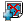
\includegraphics[width=0.7cm]{addshapefile}} To load a shapefile, start
QGIS and click on the \toolbtntwo{addshapefile}{Add a vector layer}
toolbar button\index{shapefile!loading} or simply type \keystroke{V}. This same tool can be used to
load any of the formats supported by the OGR library.

Clicking on the tool brings up a standard open file dialog (see Figure
\ref{fig:openshapefile}) which allows you to navigate the file system and load
a shapefile or other supported data source. 
The selection box \button{File of type} allows you to preselect some OGR supported file formats.

You can also select the Encoding type for the shapefile if desired.

\begin{figure}[h]
   \begin{center}
   \caption{Open an OGR Supported Vector Layer Dialog}\label{fig:openshapefile}\smallskip
   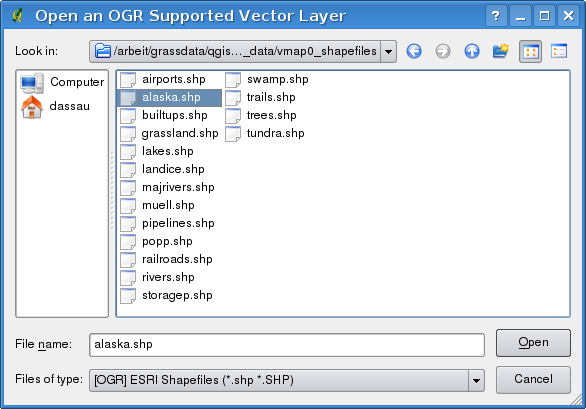
\includegraphics[clip=true, width=14cm]{shapefileopendialog}
\end{center} 
\end{figure}

Selecting a shapefile from the list and clicking \button{Open} loads it into QGIS. Figure
\ref{fig:loadedshapefile} shows QGIS after loading the \filename{alaska.shp} file.

\begin{figure}[ht]
   \begin{center}
   \caption{QGIS with Shapefile of Alaska loaded}\label{fig:loadedshapefile}\smallskip
   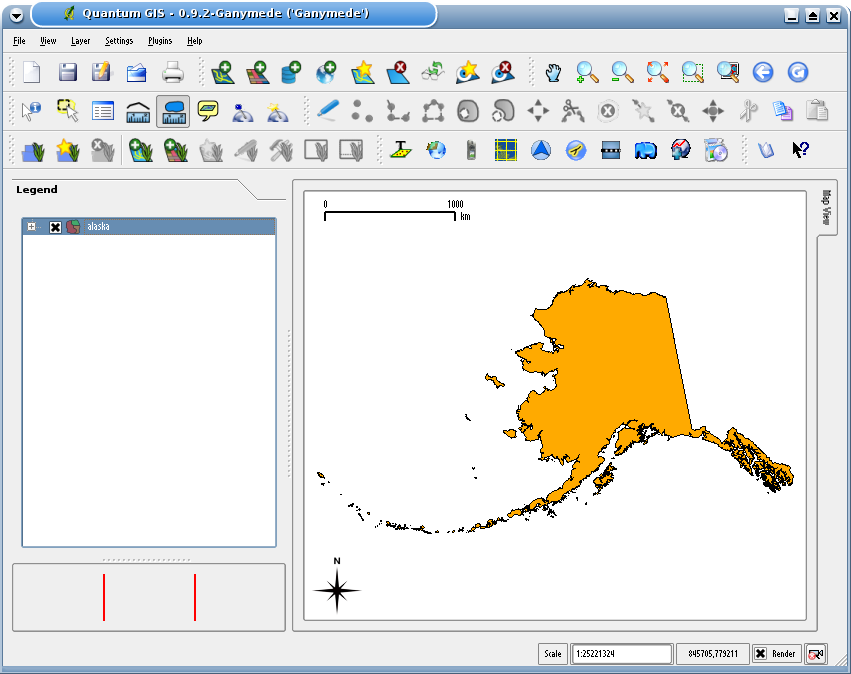
\includegraphics[clip=true, width=17cm]{shapefileloaded09}
\end{center} 
\end{figure}

\begin{Tip}\caption{\textsc{Layer Colors}}
\qgistip{When you add a layer to the map, it is assigned a random color. When
adding more than one layer at a time, different colors are assigned to each. }
\end{Tip}

Once loaded, you can zoom around the shapefile using the map navigation tools.
To change the symbology of a layer, open the \button{layer properties} dialog by double
clicking on the layer name or by right-clicking on the name in the legend and
choosing \button{Properties} from the popup menu. See
Section \ref{sec:symbology} for more information on setting symbology of
vector layers.
  
\subsubsection{Improving Performance}

To improve the performance of drawing a shapefile, you can create a spatial
index. A \index{spatial index!shapefiles} spatial index will improve the 
speed of both zooming and panning. Spatial indexes used by QGIS have a 
\filename{.qix} extension.

Use these steps to create the index:

\begin{itemize}
\item Load a shapefile.
\item Open the \button{Layer Properties} dialog by double-clicking on the
shapefile name in the legend or by right-clicking and choosing
\button{Properties} from the popup menu.
\item In the tab \tab{General} click the \button{Create} button on the Spatial
Index section.
\end{itemize}

\subsubsection{Loading a MapInfo Layer}
\index{vector layers!MapInfo}

To load a MapInfo layer, click on the \toolbtntwo{addshapefile}{Add a vector layer}
toolbar bar button or type \keystroke{V}, change the file type filter to
\fieldname{MapInfo (*.mif
*.tab *.MIF *.TAB)} and select the layer you want to load.

\subsubsection{Loading an ArcInfo Coverage}
\index{vector layers!ArcInfo Coverage}

Loading an ArcInfo coverage is done using the same method as with a
shapefiles and MapInfo layers. Click on the \toolbtntwo{addshapefile}{Add a vector layer}
toolbar button or type \keystroke{V} to open the layer dialog and change the file type filter to
\fieldname{All files (*.*)}. Navigate to the coverage directory and select one
of the following files (if present in your coverage):

\begin{itemize}
\item \filename{.lab} - to load a label layer (polygon labels or standing points).
\item \filename{.cnt} - to load a polygon centroid layer 
\item \filename{.arc} - to load an arc (line) layer.
\item \filename{.pal} - to load a polygon layer.
\end{itemize}

\subsection{PostGIS Layers}
\index{vector layers!PostGIS|see{PostGIS}}
\index{PostGIS!layers}
\label{label_postgis} 

PostGIS layers are stored in a PostgreSQL database. The advantages of PostGIS
are the spatial indexing, filtering and query capability. Using PostGIS,
vector functions such as select and identify work more accurately than with
OGR layers in QGIS.

To use PostGIS layers you must:\index{PostgreSQL!loading layers}

\begin{itemize}
\item Create a stored connection in QGIS to the PostgreSQL database (if one is
not already defined).\index{PostgreSQL!connection}
\item Connect to the database.
\item Select the layer to add to the map.
\item Optionally provide a SQL \sqltable{where} clause to define which features
to load from the layer.
\item Load the layer.
\end{itemize}

\subsubsection{Creating a stored
Connection}\index{PostgreSQL!connection}\label{sec:postgis_stored}

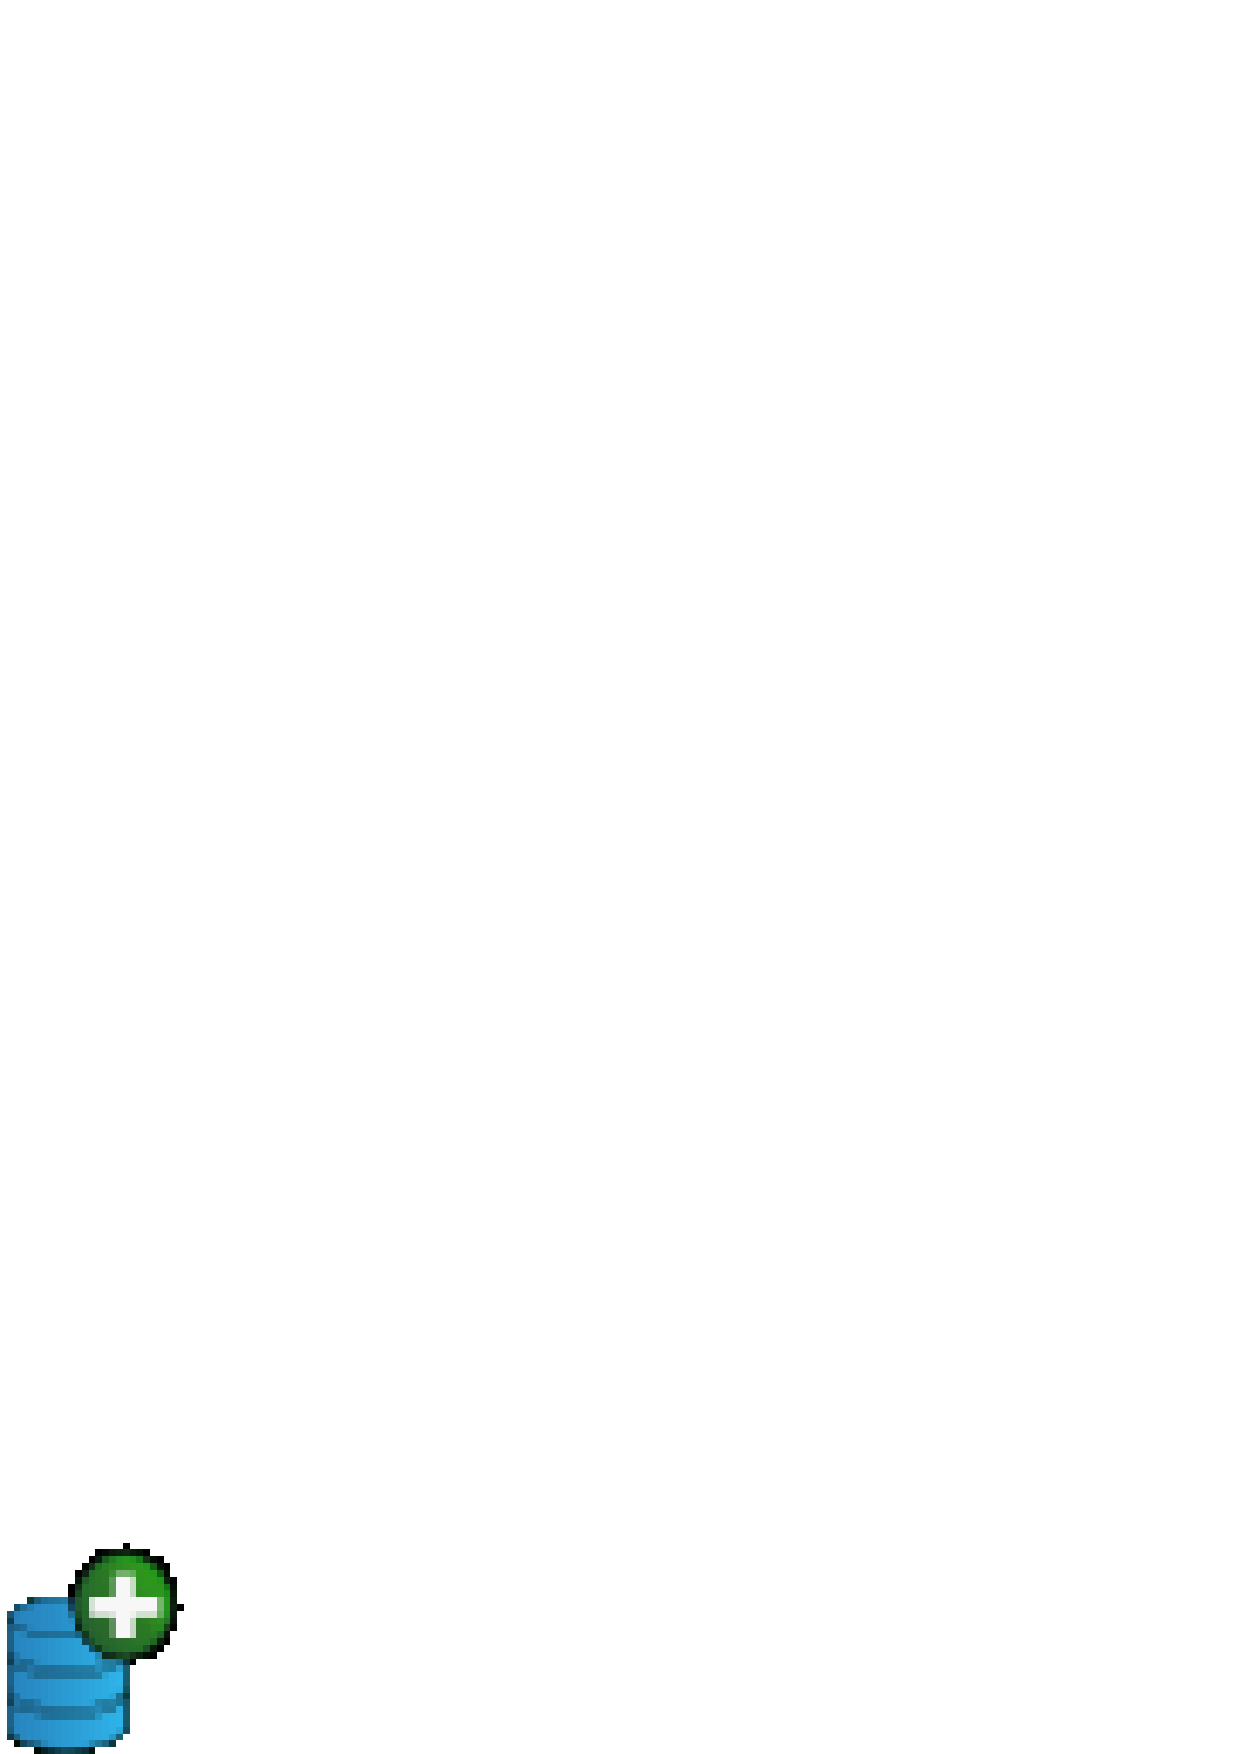
\includegraphics[width=0.7cm]{mActionAddLayer} The first time
you use a PostGIS data source, you must create a connection to the PostgreSQL
database that contains the data. Begin by clicking on the
\toolbtntwo{mActionAddLayer}{Add a PostGIS Layer} toolbar button, selecting the
\dropmenuopttwo{mActionAddLayer}{Add a PostGIS Layer...} option from the \mainmenuopt{Layer} menu or typing
\keystroke{D}. 
%FIXME: dialog macro here?
The \toolbtn{Add PostGIS Table(s)} dialog will
be displayed. To access the connection manager\index{PostgreSQL!connection
manager}, click on the \button{New} button to display the \toolbtn{Create a New
PostGIS Connection} dialog. The parameters required for a connection are shown
in table \ref{tab:postgis_connection_parms}.

\begin{table}[h]\index{PostgreSQL!connection parameters}
\centering
\caption{PostGIS Connection
Parameters}\label{tab:postgis_connection_parms}\medskip
 \begin{tabular}{|l|p{5in}|}
\hline Name & A name for this connection. Can be the same as \textsl{Database}.
\\
\hline Host \index{PostgreSQL!host}
& Name of the database host. This must be a resolvable host name the same as
would be used to open a telnet connection or ping the host. \\
\hline Database \index{PostgreSQL!database} & Name of the database.  \\
\hline Port \index{PostgreSQL!port}& Port number the PostgreSQL database
server listens on. The default port is 5432.\\
\hline Username \index{PostgreSQL!username}& User name used to login to the
database. \\
\hline Password \index{PostgreSQL!password}& Password used with
\textsl{Username} to connect to the database.\\
\hline
\end{tabular}
\end{table}

Once the parameters have been filled in, you can test the connection by
clicking on the \button{Test
Connection} button\index{PostgreSQL!connection!testing}. To save the password
with the connection information, check the \checkbox{Save Password} option.

\begin{Tip}\caption{\textsc{QGIS User Settings and
Security}}\index{settings}\index{security}
\qgistip{Your customized settings for QGIS are stored based on the operating
system. \nix, the settings are stored in your home directory in
\filename{.qt/qgisrc}. \win, the settings are stored in the registry. Depending on
your computing environment, storing passwords in your QGIS settings may be a
security risk.
}
\end{Tip}

\subsubsection{Loading a PostGIS Layer}\index{PostgreSQL!loading layers}

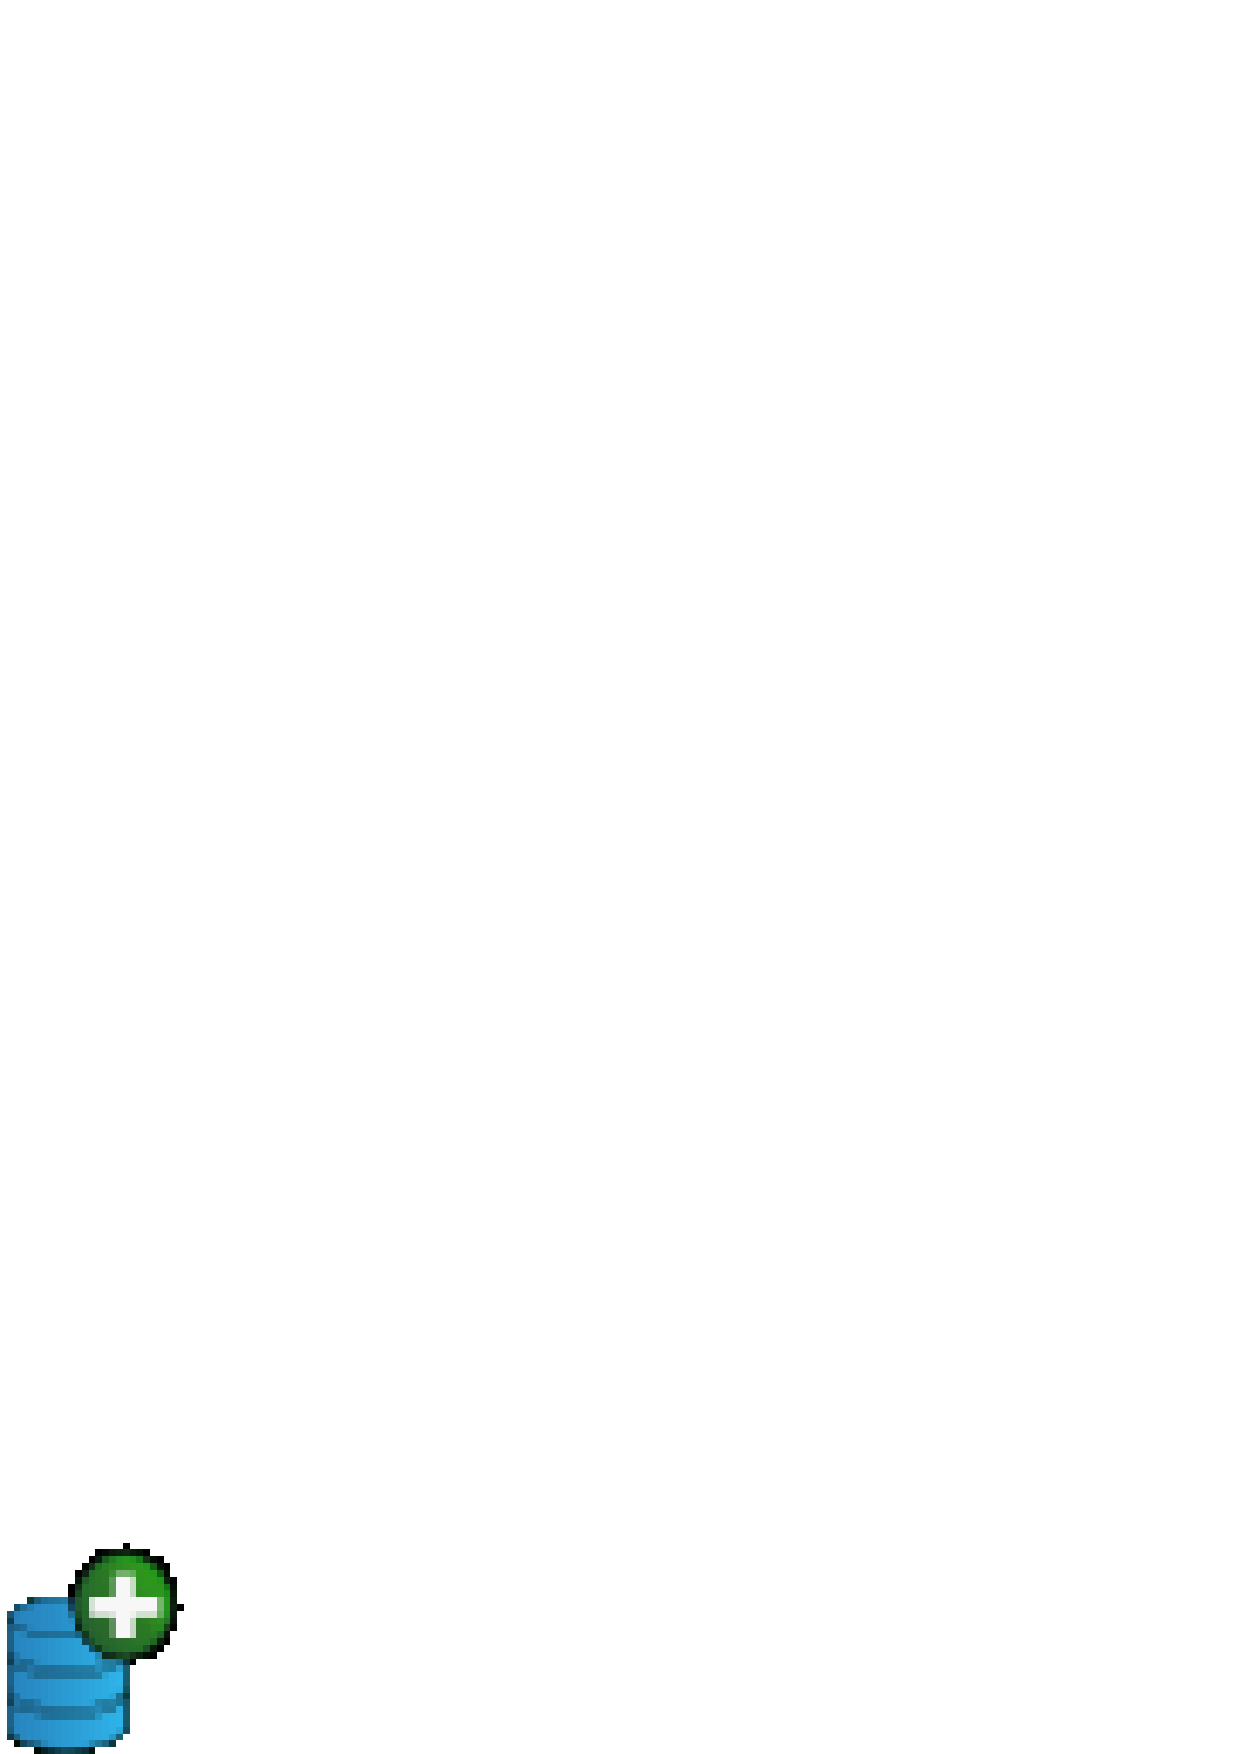
\includegraphics[width=0.7cm]{mActionAddLayer} Once you have one or more
connections defined, you can load layers from the PostgreSQL database. Of
course this requires having data in PostgreSQL. See Section
\ref{sec:loading_postgis_data} for a discussion on importing data into the
database. 

To load a layer from PostGIS, perform the following steps:

\begin{itemize}
\item If the PostGIS layer dialog is not already open, click on the
\toolbtntwo{mActionAddLayer}{Add a PostGIS Layer} toolbar button.
\item Choose the connection from the drop-down list and click \button{Connect}.
\item Find the layer you wish to add in the list of available layers.
\item Select it by clicking on it. You can select multiple layers by holding
down the \keystroke{shift} key while clicking. See Section \ref{sec:query_builder} for
information on using the PostgreSQL Query Builder to further define the layer.
\item Click on the \button{Add} button to add the layer to the map.
\end{itemize}

\begin{Tip}\caption{\textsc{PostGIS Layers}}
\qgistip{Normally a PostGIS layer is defined by an entry in the
geometry\_columns table. From version \OLD % should be 0.9.0 
on, QGIS can load layers that do not have
an entry in the geometry\_columns table. This includes both tables and views.
Defining a spatial view provides a powerful means to visualize your data. Refer
to your PostgreSQL manual for information on creating views.}
\end{Tip}

\subsubsection{Some details about PostgreSQL
layers}\label{sec:postgis_details}
\index{PostgreSQL!layer details}

This section contains some details on how QGIS accesses PostgreSQL
layers. Most of the time QGIS should simply provide you with a list of
database tables that can be loaded, and load them on request. However,
if you have trouble loading a PostgreSQL table into QGIS, the information
below may help you understand any QGIS messages and give you direction on
changing the PostgreSQL table or view definition to allow QGIS to load it.

QGIS requires that PostgreSQL layers contain a column that can be
used as a unique key for the layer. For tables this usually means
that the table needs a primary key, or have a column with a unique
constraint on it. QGIS additionally requires that this column be of
type int4 (an integer of size 4 bytes). If a table lacks these items,
the oid column will be used instead. Performance will be improved if the
column is indexed (note that primary keys are automatically indexed in
PostgreSQL). 

If the PostgreSQL layer is a view the same requirements exist, but
views don't have primary keys or columns with unique constraints on
them. In this case QGIS will try to find a column in the view that is
derived from a table column that is suitable. If one cannot be found,
QGIS will not load the layer. If this occurs, the solution is to alter
the view so that it does include a suitable column (a type of int4
and either a primary key or with a unique constraint, preferably indexed).

\subsubsection{Importing Data into PostgreSQL}\label{sec:loading_postgis_data}
\index{PostGIS!SPIT!importing data}

\minisec{shp2pgsql}
Data can be imported into PostgreSQL using a number of methods. PostGIS
includes a utility called \filename{shp2pgsql} that can be used to import shapefiles into
a PostGIS enabled database. For example, to import a shapefile named
\filename{lakes.shp}
into a PostgreSQL database named \usertext{gis\_data}, use the following command:

\begin{verbatim} 
  shp2pgsql -s 2964 lakes.shp lakes_new | psql gis_data
\end{verbatim}

This creates a new layer named \usertext{lakes\_new} in the
\usertext{gis\_data} database. The
new layer will have a spatial reference identifier (SRID) of 2964. See Section 
\ref{label_projections} for more information on spatial reference systems and
projections.
\begin{Tip}
\caption{\textsc{Exporting datasets from PostGIS}\index{PostGIS!Exporting}}
\qgistip{Like the import-tool \filename{shp2pgsql} there is also a tool to export
PostGIS-datasets into shapefiles: \filename{pgsql2shp}. This is shipped within your
PostGIS distribution.} 
\end{Tip}

\minisec{SPIT Plugin}

\includegraphics[width=0.7cm]{spiticon} QGIS comes with a
plugin named 
SPIT (Shapefile to PostGIS Import Tool)\index{PostGIS!SPIT}.
SPIT can be used to load multiple shapefiles at one time and includes support
for schemas. To use SPIT, open the Plugin Manager from the \mainmenuopt{Plugins}
menu, check the box next to the \checkbox{SPIT plugin} and click \button{OK}. The SPIT
icon will be added to the plugin toolbar\index{PostGIS!SPIT!loading}. 

To import a shapefile, click on the \toolbtntwo{spiticon}{SPIT} tool in the toolbar to open the
dialog.
You can add one or more files to the queue by clicking on the \button{Add}
button. To process the files, click on the \button{Import} button. The progress of the
import as well as any errors/warnings will be displayed as each shapefile is
processed.  

\begin{Tip}\caption{\textsc{Importing Shapefiles Containing
PostgreSQL Reserved Words}}\index{PostGIS!SPIT!reserved words}
\qgistip{If a shapefile is added to the queue containing fields that are
reserved words in the PostgreSQL database a dialog will popup showing the
status
of each field. You can edit the field names\index{PostGIS!SPIT!editing field names}
prior to import and change any that are reserved words (or change any other
field names as desired). Attempting to
import a shapefile with reserved words as field names will likely fail.}
\end{Tip} 

\minisec{ogr2ogr}
Beside \filename{shp2pgsql} and \filename{SPIT} there is another tool for feeding
geodata in PostGIS: \filename{ogr2ogr}. This is part of your GDAL installation.
To import a shapefile into PostGIS, do the following:
\begin{verbatim}
  ogr2ogr -f "PostgreSQL" PG:"dbname=postgis host=myhost.de user=postgres \
  password=topsecret" alaska.shp
\end{verbatim}

This will import the shapefile \filename{alaska.shp} into the PostGIS-database
\usertext{postgis}
using the user \usertext{postgres} with the password \usertext{topsecret} on host
\server{myhost.de}.

Note that OGR must be built with PostgreSQL to support PostGIS.
You can see this by typing
\begin{verbatim}
ogrinfo --formats | grep -i post
\end{verbatim}

\subsubsection{Improving Performance}\label{label_improve}

Retrieving features from a PostgreSQL database can be time consuming,
especially over a network. You can improve the drawing performance of
PostgreSQL layers by ensuring that a \index{PostGIS!spatial index} spatial
index
exists on each layer in the database. PostGIS supports creation of a
\index{PostGIS!spatial index!GiST} GiST
(Generalized Search Tree) index to speed up spatial searches of the data.

The syntax for creating a GiST\footnote{GiST index information is taken from the PostGIS
documentation available at \url{http://postgis.refractions.net}}
index is:

\begin{verbatim}
    CREATE INDEX [indexname] ON [tablename] 
      USING GIST ( [geometryfield] GIST_GEOMETRY_OPS );
\end{verbatim}

Note that for large tables, creating the index can take a long time. Once the
index is created, you should perform a \usertext{VACUUM ANALYZE}. See the
PostGIS documentation \cite{PostGISweb} for more information.

The following is an example of creating a GiST index:
\begin{verbatim}
gsherman@madison:~/current$ psql gis_data
Welcome to psql 8.3.0, the PostgreSQL interactive terminal.

Type:  \copyright for distribution terms
        \h for help with SQL commands
        \? for help with psql commands
        \g or terminate with semicolon to execute query
        \q to quit

gis_data=# CREATE INDEX sidx_alaska_lakes ON alaska_lakes
gis_data-# USING GIST (the_geom GIST_GEOMETRY_OPS);
CREATE INDEX
gis_data=# VACUUM ANALYZE alaska_lakes;
VACUUM
gis_data=# \q
gsherman@madison:~/current$
\end{verbatim}

\subsection{The Vector Properties Dialog}\label{sec:vectorprops}
\index{vector layers!properties dialog}

The \button{vector properties} dialog provides information about a layer, symbology
settings and labeling options. If your vector layer has been loaded from a
PostgreSQL / PostGIS datastore, you can also alter the underlying SQL for the
layer - either by hand editing the SQL on the \tab{General} tab or by
% FIXME: dialog-macro here?
invoking the \toolbtn{query builder} dialog on the \tab{General} tab. To access the
\button{Layer properties} dialog, double-click on a layer in the legend or right-click on the
layer and select \button{Properties} from the popup menu.

\subsubsection{Symbology Tab}\label{sec:symbology}
\index{vector layers!symbology}

QGIS supports a number of symbology renderers to control how
vector features are displayed. Currently the following renderers
are available:

\begin{description}
    \item[Single symbol] - a single style is applied to every
    object in the layer.\index{vector layers!renderers!single symbol}
    \item[Graduated symbol] - objects within the layer are
    displayed with different symbols classified by the values of a
    particular field.\index{vector layers!renderers!graduated symbol}
    \item[Continuous colour] - objects within the layer are
    displayed with a spread of colours classified by the numerical
    values within a specified field.\index{vector layers!renderers!continuous
color}
    \item[Unique value] - objects are classified by the unique
    values within a specified field with each value having a
    different symbol.\index{vector layers!renderers!unique value}
\end{description}

To change the symbology for a layer, simply double click on its legend 
entry and the vector layer properties dialog will be 
shown.\index{symbology!changing}.

\begin{figure}[H]
   \begin{center}
   \caption{Vector Layer Properties
Dialog}\label{fig:vector_symbology}\smallskip
   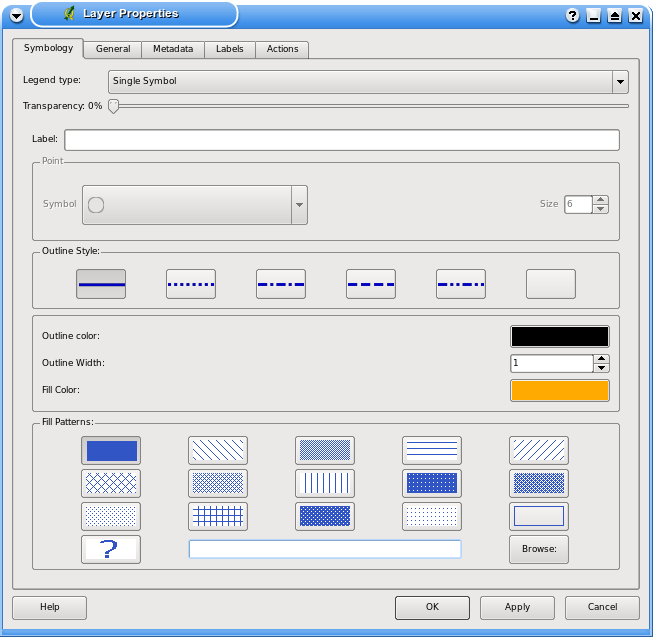
\includegraphics[clip=true, width=12cm]{vectorLayerSymbology09} 
\end{center}  
\end{figure}

Since \usertext{version v0.9} there is a function to use image files stored on your computer 
as fill pattern for vector layers.

\minisec{Vector transparency} \label{sec:vect_transparency} \index{vector layers!transparency}
QGIS \CURRENT allows to set a transparency for every vector layer. This can be done with
the slider right below the legend type (see fig. \ref{fig:vector_symbology}).
This is very useful for overlaying several vector layers.

\subsubsection{General Tab}
The \tab{General} tab is essentially like that of the raster dialog. It allows you
to change the display name, set scale dependent rendering options, create a spatial 
index of the vector file (only for OGR supported formats and PostGIS) and view or
change the projection.

The \button{Query Builder} button allows you to create a subset of the features 
in the layer - but this button currently only is available when you open the 
attribute table and select the \button{Advanced ...} button.

\subsubsection{Metadata Tab}

The \tab{Metadata} tab contains information about the layer, including specifics
about the type and location, number of features, feature type, and the editing
capabilities. The \fieldname{projection} and \fieldname{attribute} fields and 
their data type are displayed 
on this tab. This is a quick way to get information about the layer.

\subsubsection{Labels Tab}

The \tab{Labels} tab allows you to enable labeling features and control a number of
options related to placement, style and buffering.

We will illustrate this by labelling the lakes shapefile of the
\filename{qgis\_example\_dataset}:

\begin{enumerate}
\item Load the shapefiles \filename{alaska.shp} and \filename{lakes.shp} in QGIS.
\item Zoom in a bit to your favorite area with some lake.
\item Make the \filename{lakes} layer active.
\item Open the properties dialog.
\item Click on the \tab{Labels} tab.
\item Check the \checkbox{Display labels} checkbox to enable labeling.
\item Choose the field to label with. We'll use \fieldname{NAMES}.
\item Enter a default for lakes that have no name. The default label will be
  used each time QGIS encounters a lake with no value in the \fieldname{NAMES} field.
\item Click \button{Apply}.
\end{enumerate} 

Now we have labels. How do they look? They are probably too big and poorly
placed in relation to the marker symbol for the lakes.

Click on the \tab{Font Style} tab and use the \button{Font} and \button{Color}
buttons to set the font and color.

To change the position of the font relative to the feature:

\begin{enumerate} 
\item Click on the \tab{Font Alignment} tab.
\item Change the placement by selecting one of the radio buttons
in the \classname{Placement} group. To fix our labels, choose the
\button{Right} radio button.
\item Click \button{Apply} to see your changes without closing the dialog.
\end{enumerate} 

Things are looking better, but the labels are still too close to the marker. To
fix this we can use the options on the \tab{Position} tab. Here we can add
offsets for the X and Y directions. Adding an X offset of 5 will move our
labels off the marker and make them more readable. Of course if your marker
symbol or font is larger, more of an offset will be required.

The last adjustment we'll make is to \tab{buffer} the labels. This just means
putting a backdrop around them to make them stand out better. To buffer the
lakes labels:

\begin{enumerate}
\item Click the \tab{Buffer} tab.
\item Click the \checkbox{Buffer Labels?} checkbox to enable buffering.
\item Choose a size for the buffer using the spin box.
\item Choose a color by clicking on \button{Colour} and choosing your
  favorite from the color selector.
\item Click \button{Apply} to see if you like the changes.
\end{enumerate} 

If you aren't happy with the results, tweak the settings and then test again
by clicking \button{Apply}.

A buffer of 2 points seems to give a good result.
Notice you can also specify the buffer size in map units if that works out
better for you.

The remaining tabs on the \tab{Label} tab allow you control the appearance of the
labels using attributes stored in the layer. The \tab{Data} tabs allow you to
set all the parameters for the labels using fields in the layer.

\subsubsection{Actions Tab}\index{actions}\label{label_actions}

QGIS provides the ability to perform an action based on the attributes of a
feature. This can be used to perform any number of actions, for example,
running a program with arguments built from the attributes of a feature or
passing parameters to a web reporting tool.

Actions are useful when you frequently want to run an external application or
view a web page based on one or more values in your vector layer. An example
is performing a search based on an attribute value. This concept is used in 
the following discussion.

\minisec{Defining Actions}\index{actions!defining}

Attribute actions are defined from the vector layer properties dialog. To
define an action, open the vector layer properties dialog and click on the
\tab{Actions} tab. Provide a descriptive name for the action. The action
itself must contain the name of the application that will be executed when the
action is invoked. You can add one or more attribute field values as arguments
to the application. When the action is invoked any set of characters that
start with a \% followed by the name of a field will be replaced by the value of
that field. The special characters \%\% \index{\%\%}will be replaced by the value
of the field that was selected from the identify results or attribute table (see
Using Actions below).  Double quote marks can be used to group text into a
single argument to the program, script or command. Double quotes will be
ignored if preceded by a backslash.

Two example actions are shown below:\index{actions!examples}

\begin{itemize}
  \item \usertext{konqueror http://www.google.com/search?q=\%nam}
  \item \usertext{konqueror http://www.google.com/search?q=\%\%}
\end{itemize}


In the first example, the web browser konqueror is invoked and passed a URL to
open. The URL performs a Google search on the value of the \fieldname{nam} field
from our vector layer. Note that the application or script called by the
action must be in the path or you must provided the full path. To be sure, we could
rewrite the first example as: \usertext{/opt/kde3/bin/konqueror
http://www.google.com/search?q=\%nam}. This will ensure that the konqueror
application will be executed when the action is invoked.

The second example uses the \%\% notation which does not rely on a particular
field for its value. When the action is invoked, the \%\% will be replaced by
the value of the selected field in the identify results or attribute table.

\minisec{Using Actions}\index{actions!using}\label{label_usingactions}
% FIXME: dialog-macro here?
Actions can be invoked from either the \button{Identify Results} dialog or the
\toolbtntwo{mActionOpenTable}{Attribute table} dialog. To invoke an action, right click on the
record and choose the action from the popup menu. Actions are listed in the popup
menu by the name you assigned when defining the actions. Click on the action you
wish to invoke.

If you are invoking an action that uses the \%\% notation, right-click on the
% FIXME: dialog-macro here?
field value in the \button{Identify Results} dialog or the
\toolbtntwo{mActionOpenTable}{Attribute table} that you wish to pass to the application or script.

Here is another example that pulls data out of a vector layer and inserts them
into a file using bash and the \usertext{echo} command (so it will only work
\nix or perhaps \osx). The layer in question has fields for a species name
\fieldname{taxon\_name}, latitude \fieldname{lat} and longitude
\fieldname{long}. I would like to be able to
make a spatial selection of a localities and export these field values to a
text file for the selected record (shown in yellow in the QGIS map area). Here is
the action to achieve this:

\begin{verbatim}
  bash -c "echo \"%taxon_name %lat %long\" >> /tmp/species_localities.txt"
\end{verbatim} 

After selecting a few localities and running the action on each one, opening
the output file will show something like this:

\begin{verbatim}
  Acacia mearnsii -34.0800000000 150.0800000000
  Acacia mearnsii -34.9000000000 150.1200000000
  Acacia mearnsii -35.2200000000 149.9300000000
  Acacia mearnsii -32.2700000000 150.4100000000
\end{verbatim} 

As an exercise we create an action that does a Google search on the 
\filename{lakes} layer. First we need to determine the URL needed to perform a search on a
keyword. This is easily done by just going to Google and doing a simple
search, then grabbing the URL from the address bar in your browser. From this
little effort we see that the format is: \url{http://google.com/search?q=qgis},
where \fieldname{qgis} is the search term. Armed with this information, we can
proceed:

\begin{itemize}
\item Make sure the \filename{lakes} layer is loaded.
\item Open the properties dialog by double-clicking on the layer in the
  legend or right-click and choose \button{Properties} from the popup menu.
\item Click on the \tab{Actions} tab.
\item Enter a name for the action, for example \usertext{Google Search}.
\item For the action, we need to provide the name of the external program to
  run. In this case, we can use Firefox. If the program is not in
  your path, you need to provide the full path.
\item Following the name of the external application, add the URL used for
  doing a Google search, up to but not included the search term:
  \url{http://google.com/search?q=}
\item The text in the \fieldname{Action} field should now look like this:\\
  \usertext{firefox \url{http://google.com/search?q=}}
\item Click on the drop-down box containing the field names for the
  \fieldname{lakes} layer. It's located just to the right of the
  \button{Insert Field} button.
\item From the drop-down box, select \fieldname{NAMES} and click \button{Insert Field}.
\item Your action text now looks like this:\\ \usertext{firefox
  \url{http://google.com/search?q=\%NAMES}}
\end{itemize}
 
This completes the action and it is ready to use. The final text of the action
should look like this:

\begin{center}
\usertext{firefox \url{http://google.com/search?q=\%NAMES}}
\end{center}

We can now use the action. Close the properties dialog and zoom in to an area
of interest. Make sure the \filename{lakes} layer is active and identify a
lake. In the result box you'll now see that our action is visible:

\begin{figure}[H]
   \begin{center}
   \caption{Select feature and choose action}\label{fig:identify_action}\smallskip
   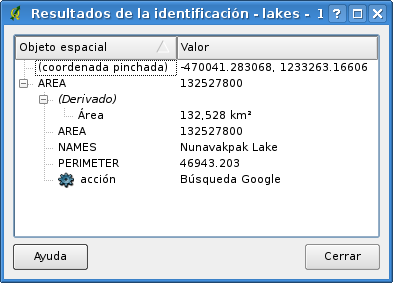
\includegraphics[clip=true, width=8cm]{identify_action} 
\end{center}  
\end{figure}

When we click on the action, it brings up Firefox and navigates to the URL
\url{http://www.google.com/search?q=Tustumena}. It is also possible to add further 
attribute fields to the action. Therefore you can add a ``+'' to the end of the action 
text, select another field and click on \button{Insert Field}. In this example there 
is just no other field available that would make sense to search for.

You can define multiple actions for a layer and each will show up in the
%FIXME: dialog macro here?
\button{Identify Results} dialog. You can also invoke actions from the attribute table
by selecting a row and right-clicking, then choosing the action from the popup
menu.

You can think of all kinds of uses for actions. For example, if you have a point layer
containing locations of images or photos along with a file name, you could
create an action to launch a viewer to display the image. You could also use
actions to launch web-based reports for an attribute field or combination of
fields, specifying them in the same way we did in our Google search example.

\subsection{Editing}\index{editing}

QGIS supports basic capabilities for editing spatial data.  Before reading any
further you should note that at this stage editing support is still preliminary.
Before performing any edits, always make a backup of the dataset you are about
to edit. 

\textbf{Note} - the procedure for editing GRASS layers is different - see
Section \ref{grass_digitising} for details.

\subsubsection{Setting the Snap Tolerance}

Before we can edit vertices, we need to set the snapping tolerance. This is the 
distance QGIS uses to \usertext{search} for the polygon and vertex you are trying to
edit when you click on the map. If you aren't within the snap tolerance,
QGIS won't find and select the vertex for editing. Tolerance is set in map
units so you may find you need to experiment to get it set right. If you
specify too big of a tolerance, QGIS may snap to the wrong vertex,
especially if you are dealing with a large number of vertices in close
proximity. Set it too small and it won't find anything and it will pop up an
annoying warning to that effect. 

To set the snap tolerance, choose \dropmenuopttwo{mActionOptions}{Project Properties} from the
\mainmenuopt{Settings} menu and click on the \tab{General} tab.  Remember the
tolerance is in map units. For our little digitizing project, the units
are in decimal degrees.  Your results may vary, but something on the order
of 0.05 to 0.1 should be fine. 

\subsubsection{Editing an Existing Layer}
\index{vector layers!editing}
\index{editing!an existing layer}
\label{sec:edit_existing_layer}

By default, QGIS loads layers read-only: This is a safeguard
to avoid accidentally editing a layer if there is a slip of the mouse.
However, you can choose to edit any layer as long as the data provider supports it,
and the underlying data source is writable (i.e. its files are not read-only).

Layer editing is most versatile when used on PostgreSQL/PostGIS data sources. 

\begin{Tip}[h]\caption{\textsc{Data Integrity}}
\qgistip{Please consider backing up your data source
before you start editing, and also at regular intervals during editing. QGIS is 
still at a pre-version 1.0 stage, and so may not be able to protect your data in all 
situations.
}
\end{Tip}

\index{Allow Editing}
All editing sessions start by choosing the \dropmenuopttwo{mActionToggleEditing}{Allow editing} option.
This can be found in the context menu after right clicking on the legend
entry for that layer.
Alternately, you can use the \index{Toggle Editing}
\toolbtntwo{mActionToggleEditing}{Toggle editing} button from the toolbar to start or stop the editing mode.\index{editing!icons}

\begin{Tip}[h]\caption{\textsc{Editing a Map is Different to Editing an Attribute Table}}
\qgistip{In this version of QGIS, the \button{Start editing}/\button{Stop editing}
couplet on the map view acts separately to the \button{Start Editing}/\button{Stop Editing}
couplet on the attribute table.
}
\end{Tip}

\begin{Tip}[h]\caption{\textsc{Save Regularly}}
\qgistip{Remember to toggle \toolbtntwo{mActionToggleEditing}{Allow editing} off regularly.  This allows you to save your changes thus far,
and also confirms that your data source can accept all
your changes.
}
\end{Tip}

\begin{Tip}[h]\caption{\textsc{Concurrent Edits}}
\qgistip{This version of QGIS does not track if somebody else is editing a feature at the same time
as you.  The last writer wins.
}
\end{Tip}

Once the layer is in edit mode, markers will appear at the
vertices.

\begin{Tip}[h]\caption{\textsc{Zoom in Before Editing}}
\qgistip{Before editing a layer, you should
zoom in to your area of interest. This 
avoids waiting while all the vertex markers are rendered across the entire layer.
}
\end{Tip}

\begin{Tip}[h]\caption{\textsc{Vertex Markers}}
\qgistip{This version of QGIS does not allow you to change the vertex markers used.
}
\end{Tip}

You can perform the following editing functions:

\begin{itemize}
\item Add Features: \toolbtntwo{mActionCapturePoint}{point},
  \toolbtntwo{mActionCaptureLine}{line} and
  \toolbtntwo{mActionCapturePolygon}{polygone}
\item \toolbtntwo{mActionMoveFeature}{Move Selected Features}
\item \toolbtntwo{mActionSplitFeatures}{Split Selected Features}
\item \toolbtntwo{mActionDeleteSelected}{Delete Selected Features}
\item \toolbtntwo{mActionAddVertex}{Add Vertex of a Feature}
\item \toolbtntwo{mActionDeleteVertex}{Delete Vertex of a Feature}
\item \toolbtntwo{mActionMoveVertex}{Move Vertex of a Feature}
\item \toolbtntwo{mActionAddRing}{Add Ring}
\item \toolbtntwo{mActionAddIsland}{Add Island}
\item \toolbtntwo{mActionEditCut}{Cut Selected Features}
\item \toolbtntwo{mActionEditCopy}{Copy Selected Features}
\item \toolbtntwo{mActionEditPaste}{Paste Selected Features}
\end{itemize}

\minisec{Adding Features}
\index{vector layers!adding!feature}

Before you start adding features, use the \toolbtntwo{mActionPan}{pan}
and \toolbtntwo{mActionZoomIn}{zoom-in}/\toolbtntwo{mActionZoomOut}{zoom-out} tools to first navigate to the area of interest.

Then you can use the \toolbtntwo{mActionCapturePoint}{Capture point},
\toolbtntwo{mActionCaptureLine}{Capture line} or
\toolbtntwo{mActionCapturePolygon}{Capture polygone} icons on the toolbar to put the QGIS cursor
into digitizing mode.

For each feature, you first digitize the geometry, then enter its attributes.

To digitize the geometry, left-click on the map area to create the
first point of your new feature.

For lines and polygons, keep on left-clicking for each additional
point you wish to capture.  When you have finished adding points,
right-click anywhere on the map area to confirm you have finished entering
the geometry of that feature.

The attribute window will appear, allowing you to enter the information for the new feature.
Figure \ref{fig:vector_digitising} shows setting attributes for a fictitious
new river in Alaska.

\begin{figure}[ht]
   \begin{center}
   \caption{Vector Digitizing Attributes Capture
Dialog}\label{fig:vector_digitising}\smallskip
   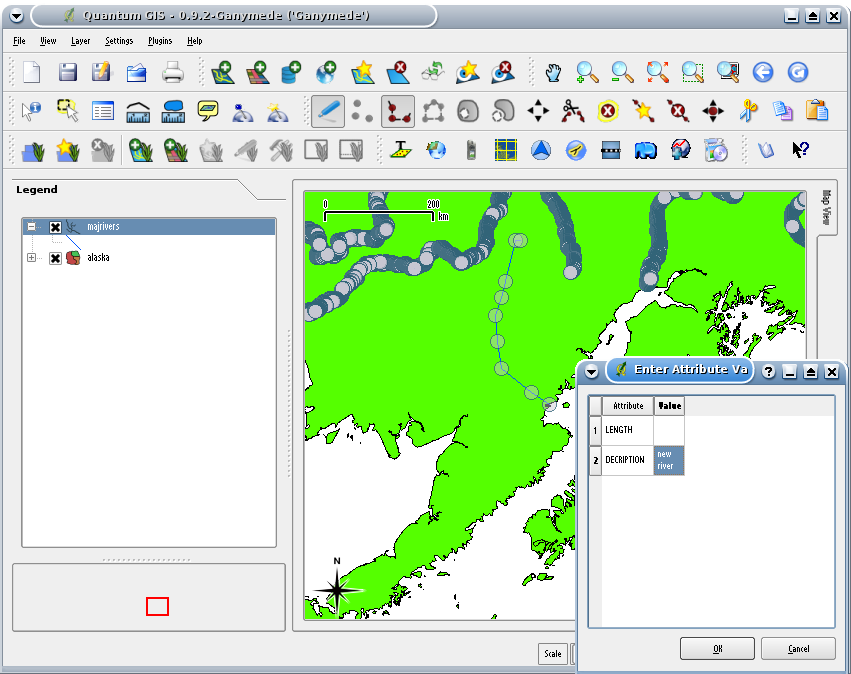
\includegraphics[clip=true, width=16cm]{digitising_attributes09}
\end{center}  
\end{figure}

\begin{Tip}[h]\caption{\textsc{Attribute Value Types}}
\qgistip{In the current version of QGIS, the attributes
dialog box does not check that the data entered matches the type expected (e.g. numeric 
vs. text). Make sure of this before pressing \button{OK}, otherwise you may find the error
will be caught later when you try to save your changes.
}
\end{Tip}

% These features will be added later
%
%\minisec{Move Selected Feature}
%\index{vector layers!move!feature}
%
%%% INPUT IS MISSING
%
%\minisec{Split Selected Feature}
%\index{vector layers!split!feature}
%
%%%% INPUT IS MISSING
%

\minisec{Editing Vertices of a Feature}
\index{vector layers!editing!vertex}

For both PostgreSQL/PostGIS and shapefile-based layers, the vertices of features can be edited. 

Vertices can be directly edited, that is, you don't
have to choose which feature to edit before you can change
its geometry.
In some cases, several features may share the same vertex
and so the following rules apply when the mouse is pressed
down near map features:

\begin{itemize}
\item \textbf{Lines}    - The nearest line to the mouse position
                          is used as the target feature.
                          Then (for moving and deleting a vertex)
                          the nearest vertex
                          on that line is the editing target.

\item \textbf{Polygons} - If the mouse is inside a polygon, then it is
                          the target feature; otherwise the nearest polygon
                          is used.
                          Then (for moving and deleting a vertex)
                          the nearest vertex
                          on that polygon is the editing target.
\end{itemize}

You will need to set the property
\mainmenuopt{Settings}>\dropmenuopttwo{mActionOptions}{Project
Properties}>\dropmenuopt{General}>\dropmenuopt{Snapping Tolerance}
to a number greater than zero.  Otherwise QGIS will not be able to tell which feature is being edited.


\minisec{Adding Vertices of a Feature}
\index{vector layers!adding!vertex}

You can add new vertices to a feature by using the
\toolbtntwo{mActionAddVertex}{Add Vertex} icon
on the toolbar.

Note, it doesn't make sense to add more vertices to a Point feature!

In this version of QGIS, vertices can only be added to an \textit{existing} line
segment of a line feature.  If you want to extend a line beyond its end,
you will need to move the terminating vertex first, then add a new vertex where
the terminus used to be.

\minisec{Moving Vertices of a Feature}
\index{vector layers!moving!vertex}

You can move vertices using the \toolbtntwo{mActionMoveVertex}{Move Vertex} icon
on the toolbar.

\minisec{Deleting Vertices of a Feature}
\index{vector layers!deleting!vertex}

You can delete vertices by using the \toolbtntwo{mActionDeleteVertex}{Delete Vertex} icon
on the toolbar.

Note, it doesn't make sense to delete the vertex of a Point feature!
Delete the whole feature instead.

Similarly, a one-vertex line or a two-vertex polygon is also
fairly useless and will lead to unpredictable results elsewhere
in QGIS, so don't do that.

\textbf{Warning:} A vertex is identified for deletion as
soon as you click the mouse near an eligible
feature.  To undo, you will need to toggle
Editing off and then discard your changes.
(Of course this will mean that other unsaved changes will be lost, too.)

\minisec{Add Ring}
\index{vector layers!add!ring}
\textbf{New since v0.9}

You can create ring polygons using the \toolbtntwo{mActionAddRing}{Add Ring}
icon in the toolbar. This means inside an existing area it is
possible to digitize further polygons, that will occur as a 'whole', so only 
the area in between the boundaries of the outer and inner polygons remain as 
a ring polygon. 

\minisec{Add Island}
\index{vector layers!add!island}
\textbf{New since v0.9}

You can \toolbtntwo{mActionAddIsland}{add island} polygons to a selected multipolygon. 
The new island polygone 
has to be digitized outside the selected multipolygon. 

% FIXME: In versions > 0.9.0 tries to convert a selected normal polygone to a
% multipolygone, if you try to use the "add island" funtionality. 
% (not yet implemented)

\minisec{Cutting, Copying and Pasting Features}
\index{vector layers!cut!feature}
\index{vector layers!copy!feature}
\index{vector layers!paste!feature}
\index{editing!cutting features}
\index{editing!copying features}
\index{editing!pasting features}

Selected features can be cut, copied and pasted between layers in the
same QGIS project, as long as destination layers are set to 
\toolbtntwo{mActionToggleEditing}{Toggle editing} beforehand.

Features can also be pasted to external applications as text:  That is,
the features are represented in CSV format with the geometry data appearing 
in the OGC Well-Known Text (WKT) format.

However in this version of QGIS, text features from outside QGIS cannot 
be pasted to a layer within QGIS.

When would the copy and paste function come in handy? Well, it turns out that 
you can edit more than one layer at a time and copy/paste features between 
layers. Why would we want to do this?  Say we need to do some work on a new 
layer but only need one or two lakes, not the 5,000 on our \filename{big\_lakes} 
layer. We can create a new layer and use copy/paste to plop the needed lakes 
into it. 

As an example we are copying some lakes to a new layer:

\begin{enumerate}
\item Load the layer you want to copy from (source layer)
\item Load or create the layer you want to copy to (target layer) 
\item Start editing for both layers 
\item Make the source layer active by clicking on it in the legend 
\item Use the \toolbtntwo{mActionSelect}{Select} tool to select the feature(s) on the source layer
\item Click on the \toolbtntwo{mActionEditCopy}{Copy Features} tool
\item Make the destination layer active by clicking on it in the legend 
\item Click on the \toolbtntwo{mActionEditPaste}{Paste Features} tool 
\item Stop editing and save the changes
\end{enumerate}

What happens if the source and target layers have
different schemas (field names and types are not the same)? QGIS populates
what matches and ignores the rest. If you don't care about the attributes
being copied to the target layer, it doesn't matter how you design the
fields and data types. If you want to make sure everything - feature and its
attributes - gets copied, make sure the schemas match.

\begin{Tip}[h]\caption{\textsc{Congruency of Pasted Features}}
\qgistip{If your source and destination layers use the
same projection, then the pasted features will have
geometry identical to the source layer.
However if the destination layer is a different projection
then QGIS cannot guarantee the geometry is identical.
This is simply because there are small rounding-off errors
involved when converting between projections.
}
\end{Tip}

\minisec{Deleting Selected Features}
\index{vector layers!deleting!feature}

If we want to delete an entire polygon, we can do that by first selecting 
the polygon using the regular \toolbtntwo{mActionSelect}{Select Features} tool. You can select 
multiple features for deletion. Once you have the selection set, use the 
\toolbtntwo{mActionDeleteSelected}{Delete Selected} tool to delete the features. There is no undo function, 
but remember your layer isn't really changed until you stop editing and choose 
to save your changes. So if you make a mistake, you can always cancel the save.

The \toolbtntwo{mActionEditCut}{Cut Features} tool on the digitizing toolbar can
also be used to delete features. This effectively deletes the feature but
also places it on a ``spatial clipboard". So we cut the feature to delete. 
We could then use the \toolbtntwo{mActionEditPaste}{paste tool} to put it back, giving us a one-level undo 
capability. Cut, copy, and paste work on the currently selected features, 
meaning we can operate on more than one at a time.

\begin{Tip}[h]\caption{\textsc{Feature Deletion Support}}
\qgistip{When editing ESRI shapefiles, the deletion
of features only works if QGIS is linked to a GDAL version 1.3.2 or greater. 
The OS X and Windows versions of QGIS available from the download site are built 
using GDAL 1.3.2 or higher.
}
\end{Tip}

\minisec{Snap Mode}
\index{editing!snap}
QGIS allows digitized vertices to be snapped to other vertices of the same layer. To 
set the snapping tolerance, go to
\mainmenuopt{Settings}>\dropmenuopttwo{mActionOptions}{Project
Properties}->\dropmenuopt{General}->\dropmenuopt{Snapping Tolerance}.
Note that the snapping tolerance is in map units.

\minisec{Saving Edited Layers}
\index{editing!saving changes}

When a layer is in editing mode, any changes remain in the memory of QGIS.
Therefore they are not committed/saved immediately to the data source or disk.
When you turn editing mode off (or quit QGIS for that matter), 
you are then asked if you want to save your
changes or discard them.

If the changes cannot be saved (e.g. disk full, or the attributes have
values that are out of range), the QGIS in-memory state is preserved.  This
allows you to adjust your edits and try again.

\subsubsection{Creating a New Layer}\label{sec:create shape}\index{editing!creating a new layer}

To create a new layer for editing, choose \toolbtntwo{mActionNewVectorLayer}{New Vector Layer} from the
\mainmenuopt{Layer} menu. 
% FIXME: dialog macro here?
The \button{New Vector Layer} dialog will be displayed as
shown in Figure \ref{fig:newvectorlayer}. Choose the type of layer (point,
line or polygon).

\begin{figure}[ht]
   \begin{center}
   \caption{Creating a New Vector Dialog}\label{fig:newvectorlayer}\smallskip
   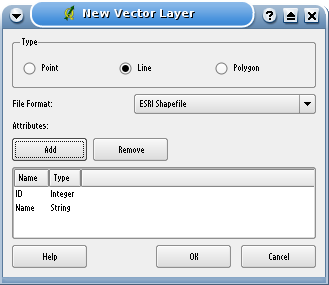
\includegraphics[clip=true, width=7cm]{newvectorlayer}
\end{center} 
\end{figure}

Note that QGIS does not yet support creation of 2.5D
features (i.e. features with X,Y,Z coordinates) or measure features. At this
time, only shapefiles can be created. In a future version of QGIS, creation of
any OGR or PostgreSQL layer type will be supported. 

Creation of GRASS-layers is supported within the GRASS-plugin. Please refer to section
\ref{sec:creating_new_grass_vectors} for more information on creating GRASS vector 
layers.

To complete the creation of the new layer, add the desired attributes by
clicking on the \button{Add} button and specifying a name and type for the
attribute. Only \fieldname{real}, \fieldname{integer}, and \fieldname{string} attributes are supported. Once you
are happy with the attributes, click \button{OK} and provide a name for the shapefile.
QGIS will automatically add a \filename{.shp} extension to the name you specify.  Once
the layer has been created, it will be added to the map and you can edit it in
the same way as described in Section \ref{sec:edit_existing_layer} above. 

\subsection{Query Builder}\label{sec:query_builder}
\index{Query Builder}

The Query Builder allows you to define a subset of a table and display
it as a layer in QGIS. It can be used for all OGR supported formats, GRASS 
files and PostGIS layers. For example, if you have a \filename{towns} layer with a
\fieldname{population} field you could select only larger towns by entering
\sqltable{population > 100000} in the SQL box of the query builder. Figure
\ref{fig:query_builder} shows an example of the query builder populated with
data from a PostGIS layer with attributes stored in PostgreSQL. 

\begin{figure}[ht]
  \begin{center}
    \caption{Query Builder}\label{fig:query_builder}\smallskip
    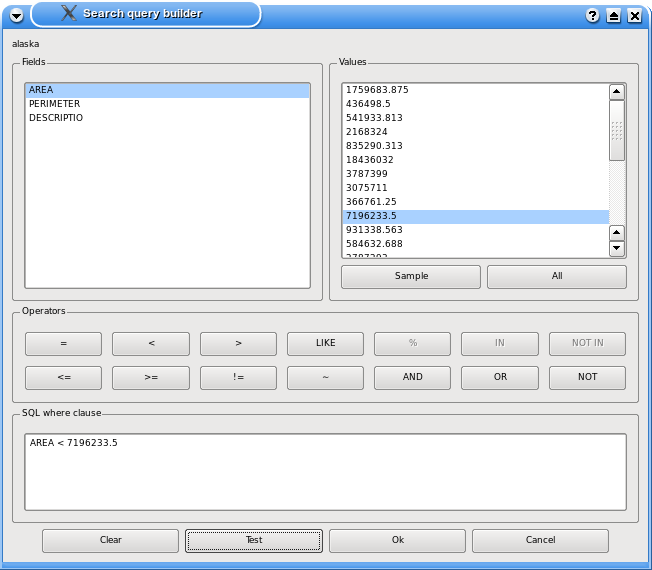
\includegraphics[clip=true, width=14cm]{querybuilder}
  \end{center}  
\end{figure}

The query builder\index{Query Builder} lists the layer's database
fields in the list box on the left. You can get a sample of the data
contained in the highlighted field by clicking on the \button{Sample} button\index{Query
Builder!generating sample list}. This retrieves the first 25 distinct values
for the field from the database. To get a list of all possible values for a
field, click on the \button{All} button\index{Query Builder!getting all
values}. To add a selected field or value to the query, double-click on
it\index{Query Builder!adding fields}. You can use the various buttons to
construct the query or you can just type it into the SQL box.

To test a query, click on the \button{Test} button\index{Query Builder!testing
queries}. This will return a count of the number of records that will be
included in the layer. When satisfied with the query, click \button{OK}. The
SQL for the where clause will be shown in the SQL column of the layer list.

\begin{Tip}\caption{\textsc{Changing the Layer Definition}}\index{Query
Builder!changing layer definitions}
\qgistip{You can change the layer definition after it is loaded by altering
the SQL query used to define the layer. To do this, open the 
%FIXME: dialog macro here?
\button{vector layer properties} dialog by double-clicking on the layer in the legend and click on the
\button{Query Builder} button on the \tab{General} tab. See Section
\ref{sec:vectorprops} for more information.}
\end{Tip}

\subsubsection{Query PostGIS layers}\label{sec:query_builder_postgis}
\index{PostgreSQL!query builder}
\index{PostGIS!query builder}
\index{query builder!PostgreSQL}
\index{query builder!PostGIS}

To query a loaded PostGIS layer there are two options. The first is to click on the 
button \toolbtntwo{mActionOpenTable}{Open Table} to open the attribute table of the PostGIS layer. Then 
click the \button{Advanced...} button at the bottom. This starts the Query Builder 
that allows to define a subset of a table and display it as described in Section 
\ref{sec:query_builder}.

The second option to query a PostGIS layer, is to open the \toolbtn{Layer Properties} 
dialog by double-clicking on the PostGIS layer name in the legend or 
by right-clicking and choosing \dropmenuopt{Properties} from the popup menu. In the tab 
\tab{General} click the \button{Query Builder} button at the bottom.

\subsubsection{Query OGR formats and GRASS files}\label{sec:query_builder_ogrgrass}
\index{OGR!query builder}
\index{GRASS!query builder}
\index{query builder!OGR}
\index{query builder!GRASS}

To query a loaded GRASS file or OGR supported format you currently need to click on the 
button \toolbtntwo{mActionOpenTable}{Open Table} to open the corresponding attribute table and click the 
\button{Advanced...} button. This starts the Query Builder and allows to define a 
subset of a table and display it as described in Section \ref{sec:query_builder}. 

The second option to start the Query Builder as decribed in Section 
\ref{sec:query_builder_postgis} is currently not supported for OGR and GRASS-layers.

\index{vector layers|)}
